\documentclass{coursework}

% Personal Information
\name{Braden}{Marshall}

% Course Information
\university{Cardiff University}
\logopath{E:/Pictures/Icons/Education/cardiffuniversity.png}
\subject{Computer Science}
\subsubject{CM3106: Multimedia}
\title{Multimedia Coursework}
\subtitle{MATLAB Interactive Fourier-based Synthesiser}
\supervisorlabel{Lecturers}
\supervisors{
	{Prof.,David,Marshall},
	{Dr.,Kirill,Sidorov},% Comment required for last element
}

% Define the file containing our references
\addbibresource{refs.bib}

\begin{document}
	\maketitlepage
	
	\tableofcontents
	
	\section{Basic Requirements}
		Throughout this section, I shall discuss the implementation of all the basic requirements I've included in my synthesiser. There are many places where we refer to the additional features, as they intertwine quite naturally with the rest of the application. For the marker's benefit, I try to leave out the details regarding additional features so they can be discussed separately. \footnote{All sources within the `\textit{+thirdparty}` package is credited to their rightful owners.}
		
		\begin{figure}[H]
			\centering
			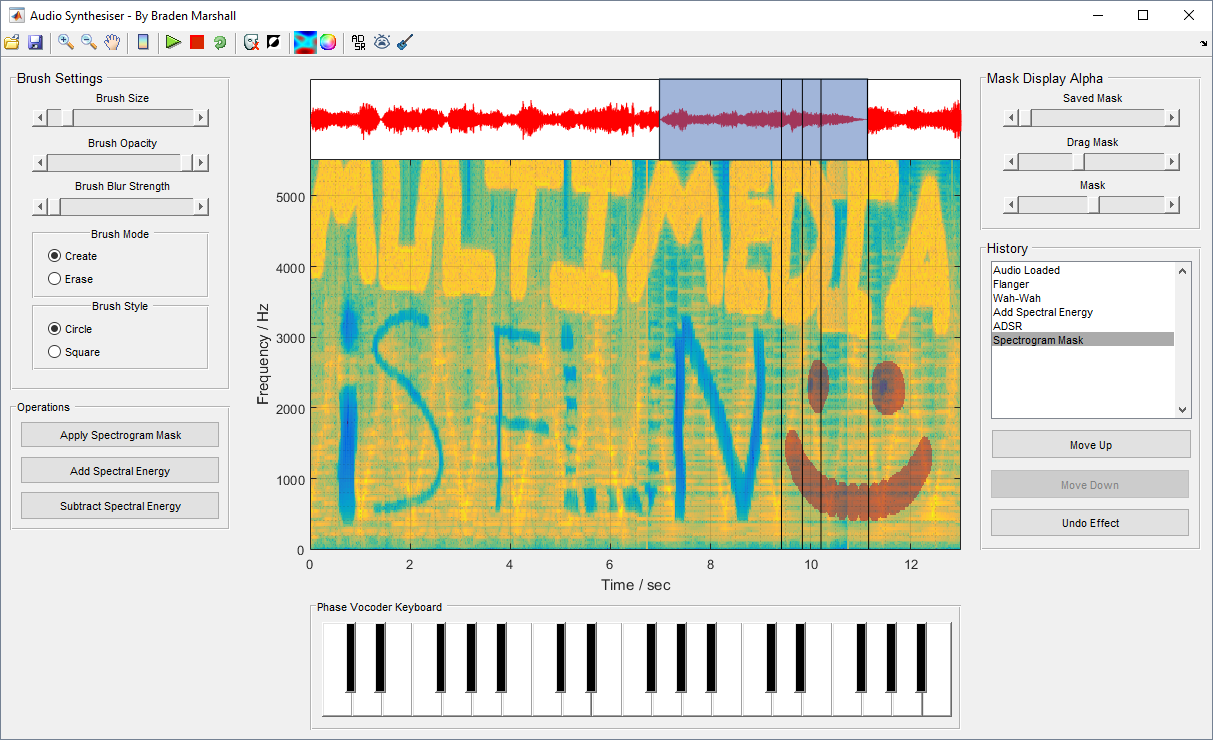
\includegraphics[max width=\textwidth]{maingui.png}
			\caption{Image of the my Synthesiser's GUI} \label{fig:image-maingui}
		\end{figure}
	
		\newpage
		
		\subsection{Synthesiser Overview}
			To launch the synthesiser, open MATLAB and add the source-code folder to the search path then run the entry-point file `\textit{synthesiser.m}`.
			
			Once the synthesiser has opened, you will notice most of the GUI components are in a disabled state. This is because an audio file has not yet been loaded. To load an audio file, click the `\textit{Open audio file}` button in the tool-bar. The majority of the GUI components should now become enabled.
			
			All the available operations should be fairly self-explanatory - keep in mind that you can learn more by hovering to reveal a tool-tip.
			
		\subsection{Spectrogram Editing}
			Upon loading some audio, you are presented with both an image of the audio signal (on top) and its spectrogram (on bottom). Editing of the spectrogram is done by creating a mask which is then applied to the spectrogram in some arbitrary way. You can create and modify your mask simply by brushing over the spectrogram image - this is done by holding your mouse down on its axes and dragging around.
			
			To the left of the spectrogram axes you will find a panel titled `\textit{Brush Settings}`. This contains a variety of configurations which alter the way in which your brush effects the mask. For example, you can change the size and shape (circle or square) of the brush.
			
			To the right of the spectrogram axes, you will see a panel titled `\textit{Mask Display Alpha}`. This allows you to modify the transparency of the mask; revealing or covering the spectrogram beneath. It is purely aesthetic and has \textbf{no} effect on the operations performed. You will notice there are three types of masks, I shall discuss these now:
			
			\begin{itemize}
				\item \textbf{Mask}: The currently buffered mask, i.e. to be used by the next mask-utilising operation.
				\item \textbf{Drag Mask}: The current brush motion, i.e. between mouse down and mouse up.
				\item \textbf{Saved Mask}: The mask which was previously used by a mask-utilising operation.
			\end{itemize}
	
			The tool-bar contains four tools directly relating to the mask and/or spectrogram. These are described below:
			\begin{itemize}
				\item \textbf{Clear Mask}: Erase the current \textit{Mask}.
				\item \textbf{Inverse Mask}: Inverse the selection of the \textit{mask}, i.e. $Mask = 1 - Mask$.
				\item \textbf{Choose Colour Map}: Display a modal of alternative colour-maps to display the spectrogram.
				\item \textbf{Select Mask Colour}: Display a modal of alternative colours to display the \textit{mask}.
			\end{itemize}
			
			The operations which utilise the mask sit to the left of the spectrogram in a panel titled `\textit{Operations}`. The only operation which was required by the basic requirements is `\textit{Apply Spectrogram Mask}`. This simply takes the pointwise product between the spectrogram and its mask, i.e. so that the unselected areas of the spectrogram are discarded.
			
			The other operations will be further discussed in \fullref{ss:spectralenergy}.
			
		\subsection{Audio Playback and the Phase Vocoder}
			There exists two ways in which you can playback the audio you've developed. One of which resides in the tool-bar, and integrates with an additional feature, which we discuss in \fullref{ss:playbackcontrol}. The other is presented in the form of a keyboard, which resides below the spectrogram image.
			
			The primary difference between the two is that the keyboard internally uses a phase vocoder to provide a greater range of sound. Middle C, that is C4, will play the audio with no additional effect. However, keys to the left will play at a higher pitched note and conversely keys to the right play at a lower pitch note.
			
		\subsection{Audio Effects}
			The following subsection will discuss ADSR volume shaping along with two additional audio effects which were implemented.
			
			\subsubsection{ADSR Volume Shaping}
				ADSR is an acronym for Attack, Decay, Sustain, Release and is a technique used to produce more natural sounds. We implement this by interpolating the audio signal's amplitude between five control points, whose position can be customised by the user.
				
				The ADSR can be accessed by pressing its corresponding button within the tool-bar, which presents the user with a modal.

			\subsubsection{Wah-Wah}
				The wah-wah is essentially a band-pass filter which is modulated over time and then mixed back in with the direct signal. This gives the effect of changing from `wwww` sounds through to `aaaahhhh` sounds.
				
				Similar to the ADSR, the wah-wah can be accessed by pressing its corresponding button within the tool-bar, which presents the user with a modal.
			
			\subsubsection{Flanger}
				The flanger is an audio effect which is produced using a comb filter - mixing two identical signals together, except applying a small delay (0ms-15ms) - and some modulation.
				
				Once again, the flanger can be accessed by pressing its corresponding button within the tool-bar, which presents the user with a modal.

	\section{Additional Features}
		Throughout this section, I shall discuss the features I have implemented which go beyond the basic specifications. This includes both entirely new functionality and drastic improvements to the basic requirements.

		\subsection{Advance User Interface}
			To make the synthesiser more of a usable application, I've invested a lot of time into the user-interface. In particular, I shall discuss three main aspects.
			
			Firstly, the variety of brush settings allow for some fairly powerful drawing to the spectrogram mask. For example, the use of opacity allows you to capture aspects of the spectrogram at different levels. This is due to the mask not being binary, but instead a floating point value between 0 and 1.
			
			I utilised this idea of opacity and implemented the ability to draw with a Gaussian blur \parencite{matlabGaussianBlur}. The user is free to control the strength of the blur as they may.
			
		\subsection{Playback Control} \label{ss:playbackcontrol}
			Within the audio signal's amplitude/time axes, the user can select particular areas of the audio signal. They are then free to loop playback of this selection using the controls available within the tool-bar.
			
			Also, certain operations are only applied on the selected slice of audio. This is extremely useful as it allows you to easily apply the same audio effect, except with different parameters, on separate, overlapping, or identical selections of audio. It also pairs very well the editable pipeline (see \ref{ss:pipeline}).
			    
		\subsection{Modular Effects and Editable Pipeline} \label{ss:pipeline}
			One of the most fundamental additional features I implemented was that of having modular effects using an editable pipeline. Conceptually, this works by recording each applied effect, and some effect data, as a node in a linked list. We are then able to pipe an audio signal through each effect in this linked list and use the output as we see fit.
			
			This allows us to have full control over the history of effects that have been applied. For example: we can apply the same effect twice, remove effects, reorder effects and even insert new effects between two existing effects.
			
			I have provided a visual representation of this pipeline to the user through the use of the listbox component. When a listbox item, i.e. an effect, is selected we set the synthesiser's state to reflect that as the current loaded audio signal. This allows the user to easily analyse the changes each effect makes.
			
			Also, it is worth noting, this maps very nicely with the real-time ability to play audio; as when the user selects a different effect the playing audio signal switches instantaneous without losing its playback position. 
			
			For performance reasons, we cache the post-effect signal at each node and reapply them only when they become stale, i.e. an alteration previously in the pipe has occurred.
			
		\subsection{Add/Subtract Spectral Energy} \label{ss:spectralenergy}
			For one of the primary features, the spectrogram mask played a fairly minor part in the overall synthesiser. Wanting to change this, I decided to try design some new operations which utilised it. I chose to try create a way in which it could be used to add/subtract energy to the selected areas; effectively allowing you to draw your own audio signal.
			
			During development, I wasn't quite sure how to justify what scaling factor should be applied to the mask before adding it to the spectrogram mask. I tried several seemingly logical values, such as: the mean, max and even a range of absolute values. None of which seemed to work.
			
			Upon investigation, I could see that the changes to the STFT were visible in the spectrogram but not the audio signal. After talking to the lab assistant, Zafi, he discovered that the ISTFT seems to scale the amplitude of the mask by the number of frequency bins.\parencite{helpZafi} Using this knowledge, I now appear to get desirable results when I multiply the scaling factor by $f/h$ - where f is the STFT's F-point FFT column count, and h is the offset.
			
		\subsection{Software Design}
			Whilst developing the synthesiser, I wanted to try learn some deeper functionality MATLAB has to offer. For the most part, this has the bonus of improving maintainability and \textit{straightforwardness} of the code. Below is a brief list of what I've done:
			
			\begin{itemize}
				\item Decoupled my code to help improve structure and organisation. This includes routing the GUI callbacks away of the entry-point file.
				\item Followed a class-base design in effort to improve maintainability and re-usability. Notably, created a class (\textit{AbstractMouse}) which makes it very easy to detect mouse interactions for \textbf{any} GUI component.
				\item Tasked the GPU to compute some more computationally extensive tasks, e.g. applying masks etc...
				\item Utilised MATLAB's \textit{inputParser} \parencite{matlabInputParser} to validate input arguments to necessary functions.
				\item Kept code up to a consistent standard, including naming conventions.
			\end{itemize}

	\printbibliography
	
\end{document}